\documentclass[10pt]{beamer}
\usetheme{Malmoe}
\setbeamertemplate{navigation symbols}{}
%\colorlet{beamer@blendedblue}{blue!40!black}
\setbeamertemplate{navigation symbols}{}
\newcommand*\oldmacro{}%
\let\oldmacro\insertshorttitle%
\renewcommand*\insertshorttitle{%
\oldmacro\hfill%
\insertframenumber\,/\,\inserttotalframenumber}

\usepackage{caption}
\usepackage{hyperref}
\usepackage[makeroom]{cancel}
\usepackage{ amssymb }
\usepackage{appendixnumberbeamer}
%\usepackage{tikz-feynman}
\usepackage{graphicx}
\begin{document}

\title{Nationwide: Telematics Assessment Exercises}
\author[Barkeloo]{Jason Barkeloo}

%\titlegraphic{\includegraphics[width=4cm]{../ATLAS-Logo-Ref-RGB.png}\hspace*{2.75cm}~%
%   \includegraphics[width=4cm]{../uo_logo_green_on_white_2.jpg}
%}

%\date{April 26, 2018}
\frame{\titlepage}
\frame{\frametitle{Table of Contents}\tableofcontents[hidesubsections]}

\frame{\frametitle{Code location for further fleshed out examples}
\begin{itemize}
\item All code for these exercises can be found via these links as ipython/jupyter notebooks located on my github in addition to attachments sent with with the presentation

\begin{itemize}
\item Part 1: \hyperlink{https://github.com/JTBarkeloo/JupyterNotebooks/blob/master/BarkelooNationwideAssessmentPart1.ipynb}{github: BarkelooNationwideAssessmentPart1.ipynp} 

\item Part 2:  \hyperlink{https://github.com/JTBarkeloo/JupyterNotebooks/blob/master/BarkelooNationwideAssessmentPart2.ipynb}{github: BarkelooNationwideAssessmentPart2.ipynp}
\end{itemize}
\end{itemize}
}

\section{Part 1: GPS Data - Analysis}
\frame{\frametitle{Tasks to be Completed}
Analysis Task:
\begin{itemize}
\item 1: Data Cleaning
\item 2: Setting of hard braking and acceleration tresholds based on the data
\item 3: Trip-by-trip Analysis and Summary
\end{itemize}

Data Set Overview:
\begin{itemize}
\item 9687 rows of 4 variables including:
\begin{itemize}
\item  trip\_id: a trip number identifier 
\item local\_dtm: a datetime timestamp of the event entry
\item latitude: latitudinal coordinate
\item longitude: longitudinal coordinate
\end{itemize}
\end{itemize}
Datasets are loaded into pandas dataframes for further analysis
}

\subsection{Task 1: Data Cleaning}

\frame{\frametitle{Data Cleaning, Gross Features}
\begin{itemize}
\item 3 Large unphysical features occur in the dataset (teleportation across the globe for 2-4 seconds)
\item These events are pruned by requiring the latitude and longitude are within $2^{\circ}$ of the median for the data set. 
\item This includes an area on the order of the state of Ohio
\begin{itemize}
\item Assumption: The sensors are used for checking daily driving habits and not long, rare, road trips.
\item No other points are removed under this cut just these large outliers but if this assumption is false (i.e. long-haul truck drivers use these) this would need to be adapted
\end{itemize}
\end{itemize}
\centering
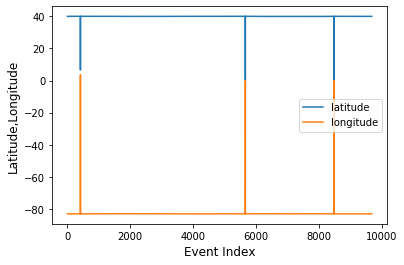
\includegraphics[width=0.5\textwidth]{Images/Image1.png}
}

\frame{\frametitle{Result of Gross Cleaning}
\begin{itemize}
\item  The median cut before leaves the longitude and latitude plots in a reasonable state.
\item Still some very fast jumps which are coincident, typically, with a change in trip\_id (GPS drift while off)
\item From this data and corresponding timestamps in local\_dtm plots of the speed $s = \frac{\Delta\text{Positions}}{\Delta\text{Time}}$ and acceleration $a = \frac{\Delta\text{Speed}}{\Delta\text{Time}}$ can be made
\end{itemize}
\centering
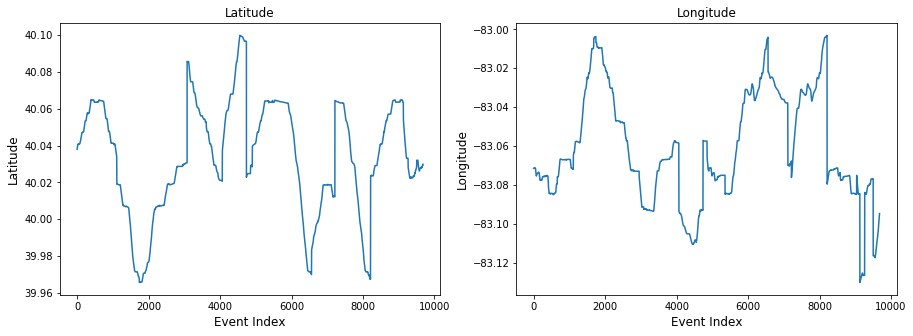
\includegraphics[width=1.\textwidth]{Images/Image2.png}
}

\frame{\frametitle{Further Cleaning - $\Delta$Position, $\Delta$Time, Speed, Acceleration}
\centering
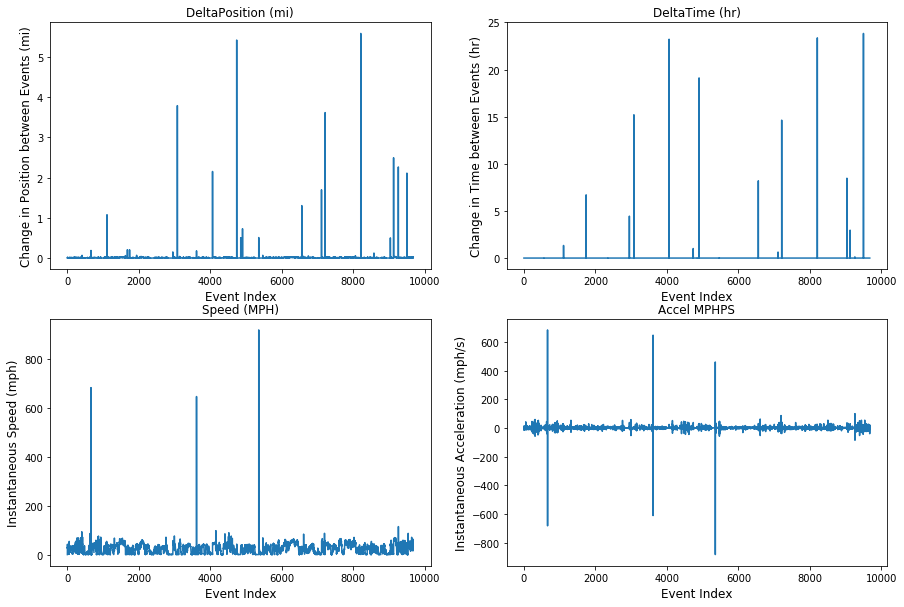
\includegraphics[width=1.\textwidth]{Images/Image3.png}
}

\frame{\frametitle{More Features to be Cleaned}
\begin{itemize}
\item From $\Delta$Position, $\Delta$Time we see the large number of drifts which account for the gps drift from trip differences
\item 15 events: These jumps will not be an issue when analyzing trip by trip as the change in position starts from the first point of the trip
\item Speed and Acceleration plots show an additional 3 further unphysical events.  These are resultant from small gps errors for a few seconds and need to be dealt with
\item Another issue comes when $\Delta$Time between two events is 0 i.e., if the frequency drops below 1Hz and two readings are taken within a second.
\begin{itemize}
\item 24 events: A 0th order approach is taken to these points and only the first is kept.  An alternative would be averaging the latitude/longitude for those points.  This would be a change within the same second and as such will not have much of an effect that isnt then averaged out in the acceleration
\end{itemize}
\end{itemize}
}

\frame{\frametitle{}
\begin{itemize}
\item
\end{itemize}
\centering
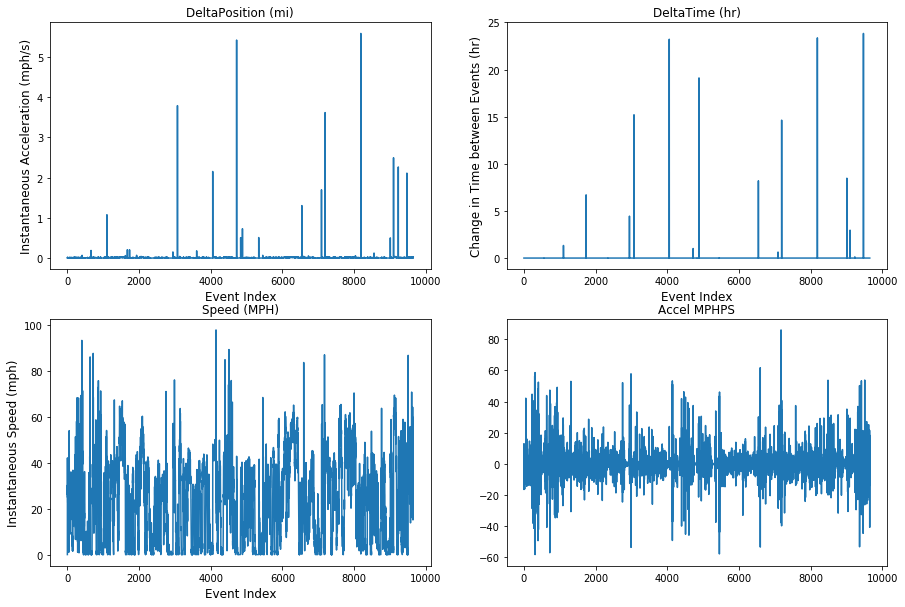
\includegraphics[width=1.\textwidth]{Images/Image4.png}
}

\frame{\frametitle{}
\begin{itemize}
\item
\end{itemize}
\centering
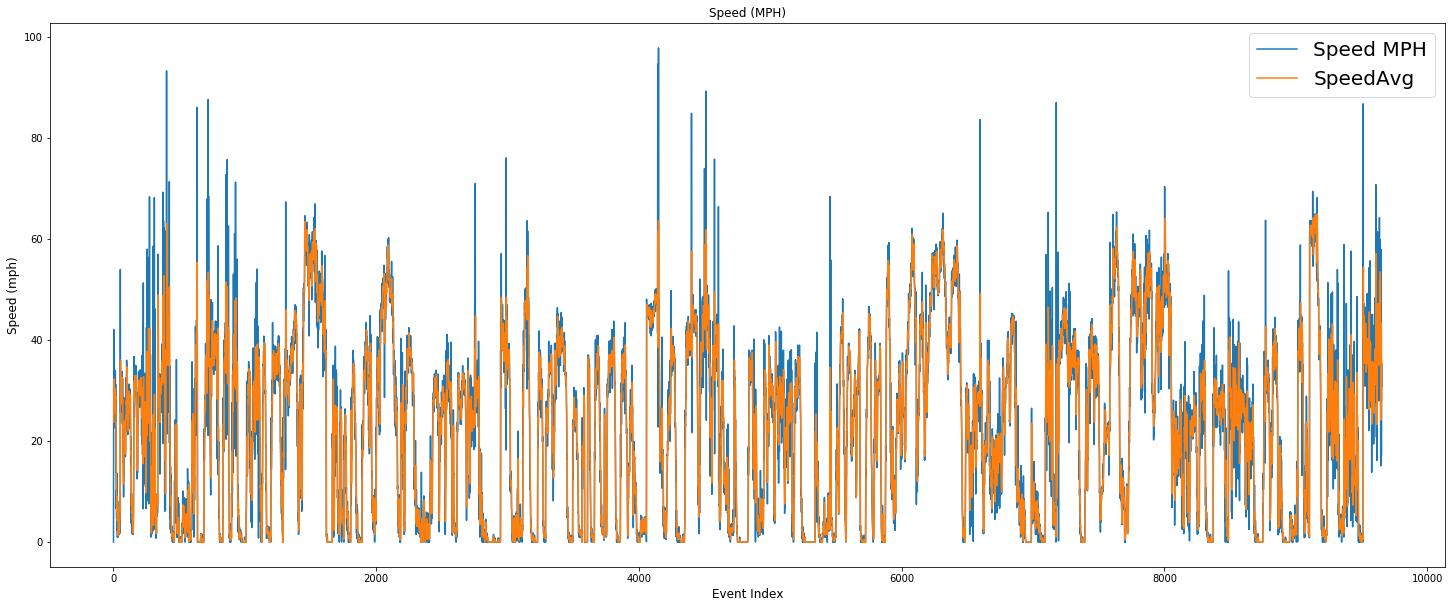
\includegraphics[width=1.\textwidth]{Images/Image5.png}
}

\frame{\frametitle{}
\begin{itemize}
\item
\end{itemize}
\centering
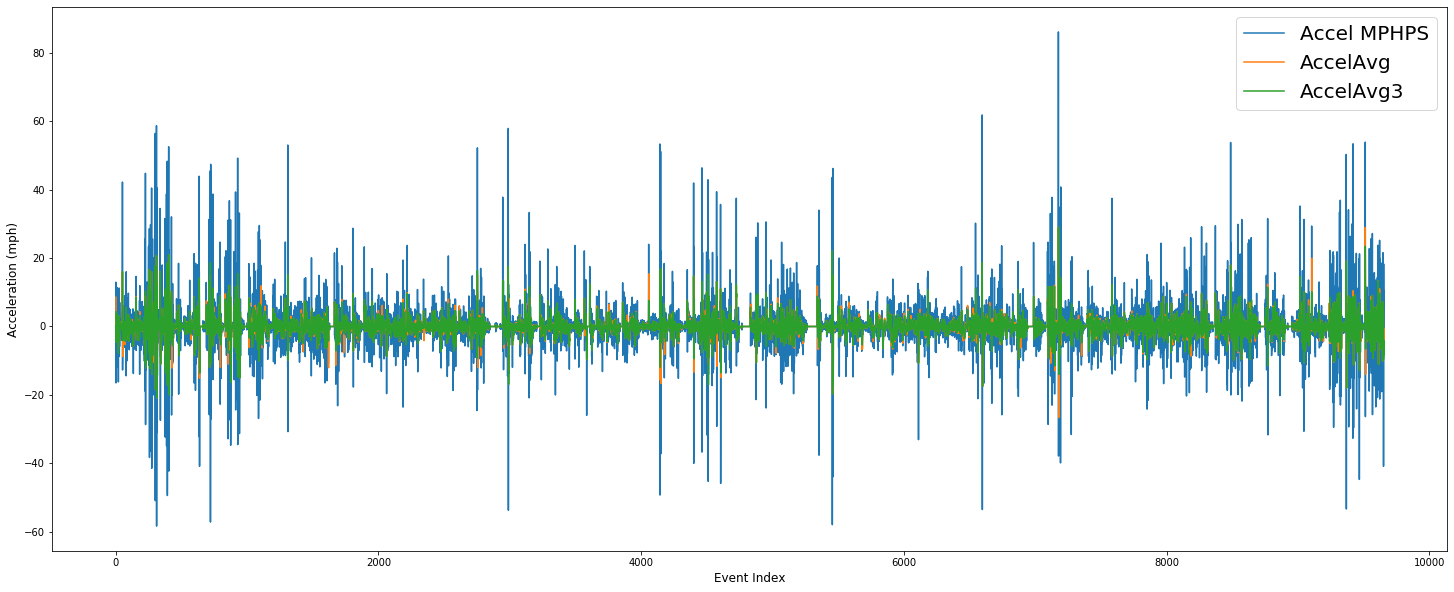
\includegraphics[width=1.\textwidth]{Images/Image6.png}
}

\frame{\frametitle{}
\begin{itemize}
\item
\end{itemize}
\centering
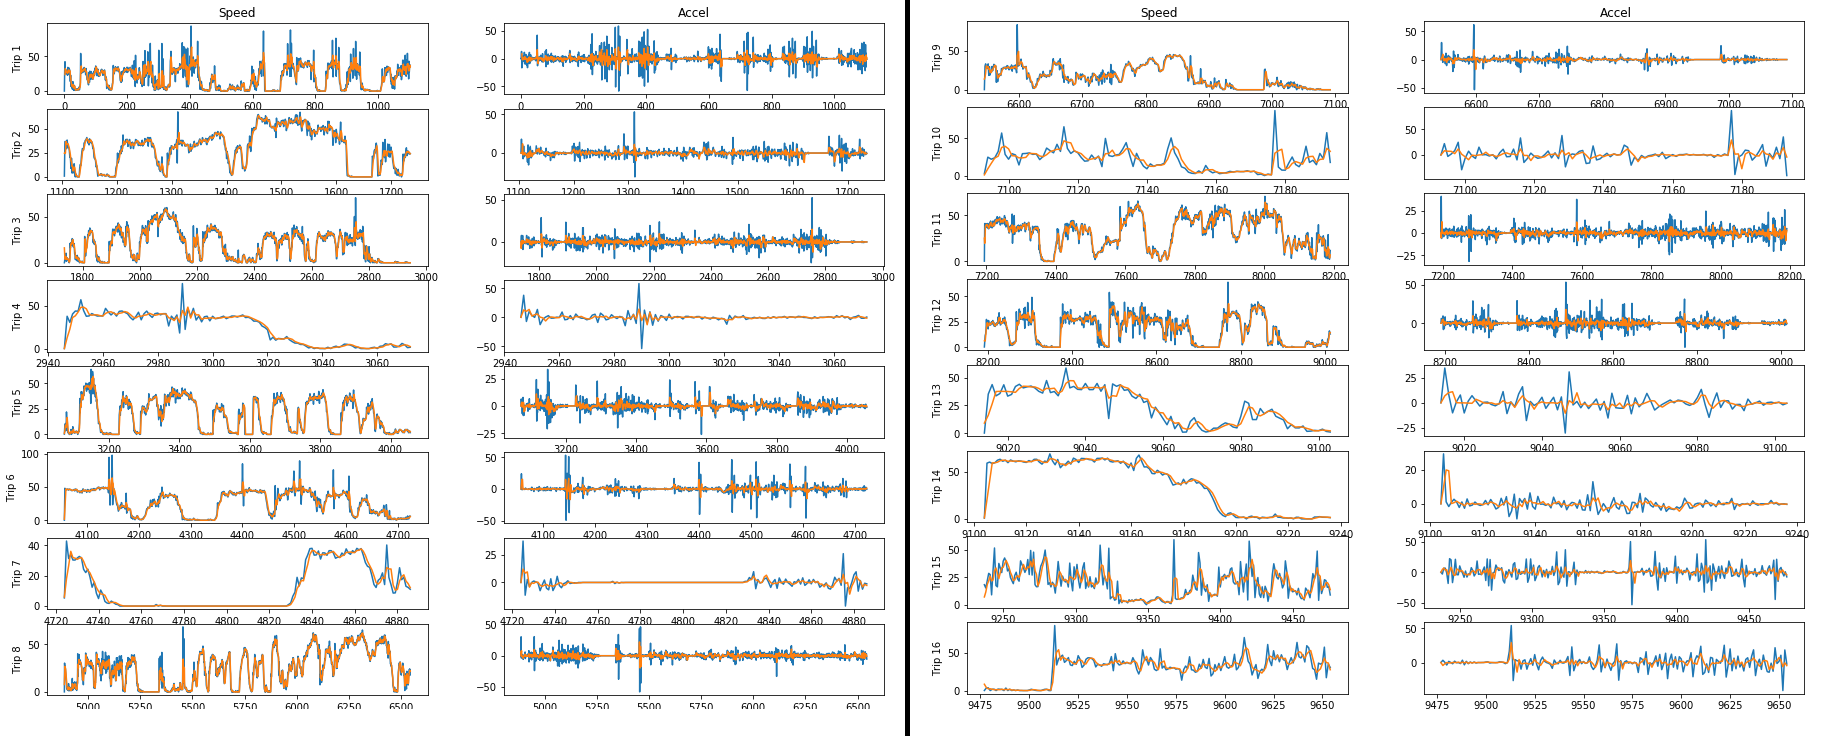
\includegraphics[width=1.\textwidth]{Images/Image7.png}
}

\frame{\frametitle{}
\begin{itemize}
\item
\end{itemize}
\centering
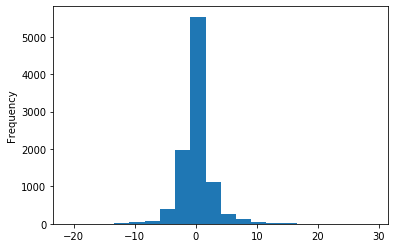
\includegraphics[width=0.5\textwidth]{Images/Image8.png}
}

\frame{\frametitle{}
\begin{itemize}
\item
\end{itemize}
\centering
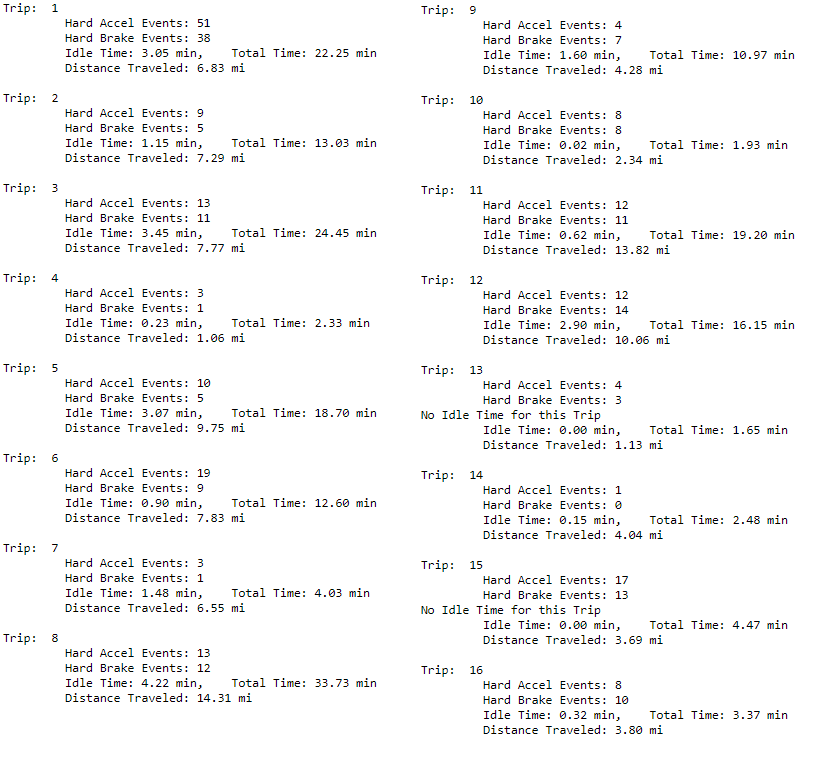
\includegraphics[width=0.7\textwidth]{Images/Image9.png}
}


\frame{\frametitle{FCNC: What are we looking for? $t\bar{t}\rightarrow W (\rightarrow l \nu) b+ q\gamma$}
\begin{itemize}
\item Final state topology
	\begin{itemize}
	\item One Neutrino, from W
	\item One Lepton, from W
	\item One B-jet, SM top
	\item \textbf{One Photon, FCNC Top}
	\item One Jet, FCNC Top
	\end{itemize}
\end{itemize}
}

\frame{\frametitle{Background Processes}
\begin{itemize}
\item Due to all of the processes at hadron colliders it is important to model similar event topologies well.
\item Major backgrounds include $t\bar{t}$, W+Jets, Z+Jets, + processes with an associated photon
\end{itemize}
%\centering
%\includegraphics[width=0.7\textwidth]{../../ThesisImages/backgrounds.png}
}

\frame{\frametitle{Monte Carlo Generation}
\begin{itemize}
\item All of our MC data is put through a showering algorithm for propagation from final decay states
\item Various showering algorithms are used at ATLAS - Pythia, Herwigg, etc.
\item All of these will add radiative photons
\item These events can be contained in other samples with explicit photons originating from the hard interaction
\item Need to remove these events or risk double counting events
\end{itemize}

}


%%%%%%%%%%%%%%%%%%%%%%%%%%%%%%%%%%%%%%%%%%%%%%%%%%%%%%%%%%%%%%%%%
\section{Part 2: Modeling}

\subsection{Object Preselection Cuts}

\frame{\frametitle{}
\begin{itemize}
\item
\end{itemize}
%\centering
%\includegraphics[width=0.7\textwidth]{../../ThesisImages/backgrounds.png}
}

\frame{\frametitle{Object Preselection}
\begin{itemize}
\item We preselect events with objects that look like our expected topology
\item Reminder that I require:
	\begin{itemize}
	\item Exactly one lepton (e or $\mu$) $\geq$ 28 GeV
	\item Exactly one Good photon $\geq$ 25GeV
	\item Missing Transverse Energy $\geq$ 30GeV
	\item $\geq 2$ Jets (at least one being b-tagged)
	\end{itemize}
\item All following plots will have signal scaled to $0.2\%$ of nonallhadronic $\sigma_{t\bar{t}}$, MC scaled to $36.07fb^{-1}$
\item Only electron channel shown.  Similar results for the muon channel are seen.
\end{itemize}
}


\subsection{Analysis}

\frame{\frametitle{Background Processes}
\begin{itemize}
\item Due to all of the processes at hadron colliders it is important to model similar event topologies well.
\item Major backgrounds include $t\bar{t}$, W+Jets, Z+Jets, + processes with an associated photon
\end{itemize}
%\centering
%\includegraphics[width=0.7\textwidth]{../../ThesisImages/backgrounds.png}
}
%%%%%%%%%%%%%%%%%%%%%%%%%%%%%%%%%%%%%%%%%%%%%%%%%%%%%%%%%%%%%%%%%%
\subsection{Model Building}

\frame{\frametitle{Background Processes}
\begin{itemize}
\item Due to all of the processes at hadron colliders it is important to model similar event topologies well.
\item Major backgrounds include $t\bar{t}$, W+Jets, Z+Jets, + processes with an associated photon
\end{itemize}
%\centering
%\includegraphics[width=0.7\textwidth]{../../ThesisImages/backgrounds.png}
}
\subsection{Data Set Enhancement}

\frame{\frametitle{Background Processes}
\begin{itemize}
\item Due to all of the processes at hadron colliders it is important to model similar event topologies well.
\item Major backgrounds include $t\bar{t}$, W+Jets, Z+Jets, + processes with an associated photon
\end{itemize}
%\centering
%\includegraphics[width=0.7\textwidth]{../../ThesisImages/backgrounds.png}
}

\section{Conclusion}
\frame{\frametitle{Conclusion, Outlook}
\begin{itemize}
\item Orthogonal validation/control regions are in development
\item Data grid run complete, need to incorporate into CR/VR plots
\item Next grid run will include a couple of looser regions for CR/VRs 
	\begin{itemize}
	\item 0 Photon Samples for Backgrounds with no Real Photons
	\item 0 BJet Samples - possibly for WJets region
	\end{itemize}
\item Top Group - Pushing for MVA, want to start investigations using these techniques 
\end{itemize}
}


%%%%%%%%%%%%%%%%%%%%%%%%%%%%%%%%%%%%%%%%%%%%%%%%%%%%%%%%%%%%%%%%
%%%%%%%%%%%%%%%%%%%%%%%%%%%%%%%%%%%%%%%%%%%%%%%%%%%%%%%%%%%%%%%% 	
\appendix
\section{Backup}
\frame{\frametitle{Backup}
}
\end{document}

%36.070
